\documentclass[12pt, a4paper]{article}%,twocolumn %pour deux colonnes mais il faut changer dautre choses aussipour que ca rend bien et avec deux colonnes on reduit notre rappport de 33 pages a 20 pages 
\usepackage[T1]{fontenc}
\usepackage[utf8]{inputenc}

\usepackage{parskip}  %pour paragraphs
\setlength{\parindent}{15pt}
\usepackage{fourier}
\usepackage{afterpage}
\usepackage[cmex10]{amsmath}
\usepackage{amssymb}
\usepackage[pdftex]{graphicx}
\usepackage{epstopdf}
\epstopdfsetup{update}
\usepackage{fancyhdr}
\usepackage[twoside, margin=2.5cm, bindingoffset=0.0cm]{geometry}
\usepackage{url}
\usepackage{siunitx}
\usepackage{float}

\usepackage[caption = false]{subfig}
\usepackage{alphalph}
\renewcommand*{\thesubfigure}{%
\alphalph{\value{subfigure}}%
}%

%\sisetup{detect-all,input-product=*}%
% \usepackage[labelformat=simple]{subcaption}
% \captionsetup{font={footnotesize,sf},skip=2pt}

% \usepackage[%backend=biber,
% style = ieee,
% sorting=none
% ]{biblatex} %,bibstyle=ieeehttps://www.overleaf.com/project/624dc5f129c1767e8bb8de67
% \addbibresource{biblio.bib}
% \renewbibmacro*{date}{%
%   \iffieldundef{year}
%     {\bibstring{nodate}}
%     {\printdate}
% }
%\usepackage{svg}
\usepackage[inkscapeformat=png]{svg}
\usepackage{tikz}
\usetikzlibrary{matrix,calc}
\DeclareMathOperator{\sech}{sech}

\usepackage[%backend=biber,
style = ieee,
sorting=none,
% style=authoryear-icomp,
% maxbibnames=9,
% maxcitenames=1,
]{biblatex} %,bibstyle=ieeehttps://www.overleaf.com/project/624dc5f129c1767e8bb8de67

\addbibresource{biblio.bib}
\renewbibmacro*{date}{%
  \iffieldundef{year}
    {\bibstring{nodate}}
    {\printdate}
}

\usepackage{hyperref} %For hyperlinks 
\hypersetup{pdfborder=0 0 0}
\usepackage[french]{babel} %language correction
\usepackage{romannum}
\usepackage{perpage}
\usepackage{csquotes}
\MakePerPage{footnote}

\usepackage{indentfirst}

%%%%%%%%%%%%%%%%%%%%%%%%%%%%%%
%For glossaries 
%%%%%%%%%%%%%%%%%%%%%%%%%%%%%%

%\usepackage{glossaries}
%\usepackage{glossary-mcols}
%\makeglossaries
%\renewcommand*{\glspostdescription}{} % Removes dots at the end of each entry.

%\DeclareGraphicsRule{.wmf}{bmp}{}{}% declare WMF filename extension
\graphicspath{{Figures/}}

\usepackage{chngcntr}
\counterwithin{figure}{section} %changer a subsection 

%%%%%%%%%%%%%%%%%%%%%%%%%%%%%%
%POUR LES CODES
%%%%%%%%%%%%%%%%%%%%%%%%%%%%%
%https://www.overleaf.com/learn/latex/Code_listing
\usepackage{listings}
\usepackage{xcolor}
\usepackage[section]{placeins}
\usepackage{enumitem}
\usepackage{accsupp}

\newcommand{\noncopynumber}[1]{%
    \BeginAccSupp{method=escape,ActualText={}}%
    #1%
    \EndAccSupp{}%
}

\definecolor{codegreen}{rgb}{0,0.6,0}
\definecolor{codegray}{rgb}{0.5,0.5,0.5}
\definecolor{codepurple}{rgb}{0.58,0,0.82}
\definecolor{backcolour}{rgb}{0.95,0.95,0.92}

\lstdefinestyle{mystyle}{
    backgroundcolor=\color{backcolour},   
    commentstyle=\color{codegreen},
    keywordstyle=\color{magenta},
    numberstyle=\tiny\color{codegray},
    stringstyle=\color{codepurple},
    basicstyle=\ttfamily\footnotesize,
    breakatwhitespace=false,         
    breaklines=true,                 
    captionpos=b,                    
    keepspaces=true,                 
    numbers = left,
    numberstyle=\tiny\noncopynumber,
    numbersep=5pt,                  
    showspaces=false,                
    showstringspaces=false,
    showtabs=false,                  
    tabsize=2
}
\lstset{style=mystyle}

%\begin{lstlisting}[language=Python, caption=Python example]
%VOtre Code
%\end{lstlisting}
%\lstinputlisting[language=Octave]{BitXorMatrix.m}%pour importer directement dun fichier

% \usepackage{physics}
\usepackage{booktabs}
% \usepackage{subfig}

%%%%%%%%%%%%%%%%%%%%%%%%%%%%%%%%%%%%%%%%%%%%%%%%%%
%Des Raccourcies
%%%%%%%%%%%%%%%%%%%%%%%%%%%%%%%%%%%%%%%%%%%%%%%%%%
\newcommand{\comment}[1]{}%pour faire des comentaires a plusueures lignes 
\usepackage{xstring}
\newcommand{\AncaBelme}{Anca Belme}
\newcommand{\AncaBELME}{Anca BELME}
\newcommand{\ijlrd}{Institut Jean le Rond $\partial ' \textrm{Alembert}$ \space}
\newcommand{\JeanCamilleChassaing}{Jean-Camille Chassaing}
\newcommand{\JeanCamilleCHASSAING}{Jean-Camille CHASSAING}
\newcommand{\RemyCornaggia}{Rémi Cornaggia}

\fancypagestyle{firstpage}{
\setlength{\headheight}{60pt}
\fancyhead[L]{
\includegraphics[height=0.1\textwidth]{SORBONNE_FAC_SCIENCES_DEF_CMJN.png}
              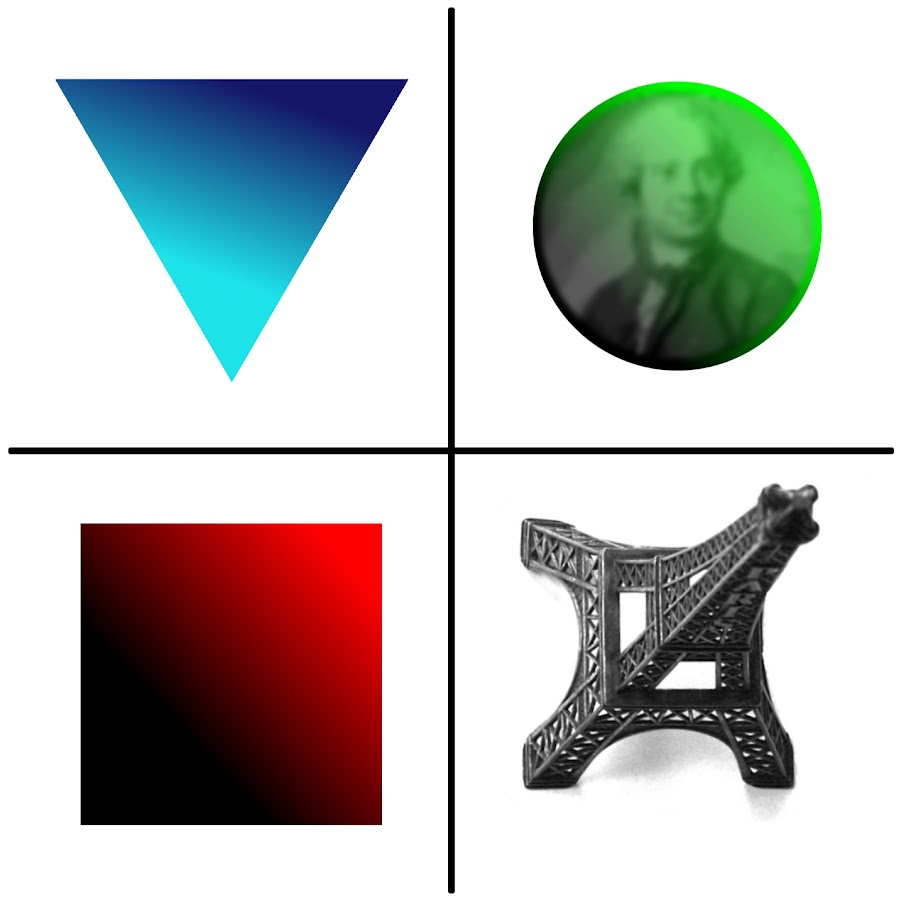
\includegraphics[height=0.1\textwidth]{Figures/logo_minimal_institut_jean_le_rond_dalembert.jpg}}
\fancyhead[R]{{\Large{ 3\up{e} }}}%semestre de l'année universitaire 2021-2022\\L1 CMI Mécanique}}}
\fancyfoot{}}

%\setlength{\parindent}{0pt}
\setlength{\parskip}{2ex plus 1ex minus 1ex}

\newcommand{\HeaderDeReapport}{Rapport de Stage}% Erdi ÇAN}
\newcommand\blankpage{%
    \null
    \thispagestyle{empty}%
    \addtocounter{page}{-1}%
    \newpage
}
  
\usepackage{atbegshi,picture}
\usepackage{lipsum}


\AtBeginShipoutNext{\AtBeginShipoutUpperLeft{%
  \put(\dimexpr\paperwidth-1cm\relax,-3cm){\makebox[0pt][r]{\Large Cursus de Master en Ingénierie  $3^{\textrm{e}}$ année }}%\framebox{Copyright DTV}}}%
}}


\begin{document}

% TODO 
% \begin{itemize}
%     \item turbulence le developper avec les statistiques de plus grande ordre unpeut plus de detail et choses fait 
%     \item Les modeles et les developper 
%     \item annexe 
%     \begin{itemize}s
%         \item autre choses fait 
%         \item derniere semaine coup doeil sur le programme de ptv 
%         \item simultaion sph avec dualsphysics
%         \begin{itemize}
%             \item pourquoi ca a pas marche 
%             \item comparisons avec des resultats mais il ya pas de beses de donnees testable cest de meme raison que on nest pas alle plus loin avec la simulation avec le manque de donnees et deja que on a des problemes avec 74 points. 
%         \end{itemize}
%     \end{itemize}
%     \item conclusion
% \end{itemize}
% \newpage

\vspace{250pt}
\title{
    \normalsize\bfseries{\HeaderDeReapport}\\
    \vspace{10pt}
    \Large\bfseries TODO
    %\vspace{10pt}
    %\textit{Intermediate Report}}
}

\author{Erdi ÇAN\\Encadré par \AncaBELME \\ Enseignant référent : \JeanCamilleCHASSAING}
\date{10 septembre 2023}
\maketitle

\tikz[remember picture, overlay] %
\node[shift={(1cm,-1cm)}] at (current page.north west) %
[anchor=north west] %
{
\includegraphics[height = 2cm]{Figures/SORBONNE_FAC_SCIENCES_DEF_CMJN.png}};

\tikz[remember picture, overlay] %
\node[shift={(6.5cm,-1cm)}] at (current page.north west) %
[anchor=north west] %
{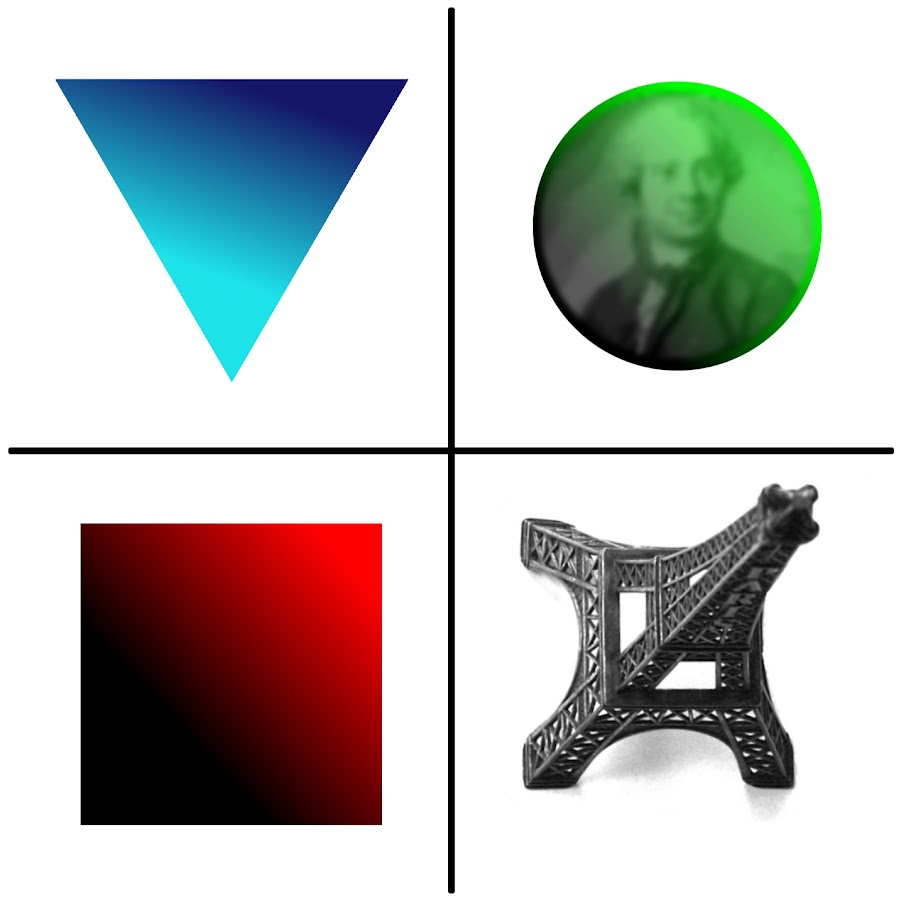
\includegraphics[height = 2cm]{Figures/logo_minimal_institut_jean_le_rond_dalembert.jpg}};


\begin{figure}[H]
    % \centering
    % \includegraphics[width = \textwidth]{Figures/image_represantation_schematique.png}
    % \caption{Representation schématique de l'environnement rude le quel les hydroliennes sont situe\autocite{title_fig}}
\end{figure}  
\thispagestyle{empty}

% \comment{
%     \vspace{1cm}
%     \begin{tabular}{m{6cm} m{5cm} m{3cm}}
%                      %\hline
%                      % after \\: \hline or \cline{col1-col2} \cline{col3-col4} ...
%                      %\bfseries{Report Type:} & Final & \\\\\\
%                      %\bfseries{Les étudiants} & Erdi ÇAN & \\\\\\
%                      %\bfseries{Thesis Director:} & Prof. Christian Enz & \dotfill{} \\\\\\
%                      \bfseries{Diercteur de recherche } & ... & %\dotfill{} \\\\\\
%                      %\bfseries{Date:} & \today  \\\\\\
%      %               \hline
%                    \end{tabular}%
% }
%\afterpage{\blankpage}
\newpage
\setcounter{page}{1}
\pagestyle{fancy}
\fancyhead{} % Clear all header fields
\setlength{\headheight}{24pt}
%\fancyhead[LE,RO]{\thepage} %
\fancyhead[CE,CO]{\HeaderDeReapport} %
\fancyfoot{} % Clear all footer fields
\fancyfoot[RE,LO]{\thepage}
%\fancyfoot[RE,LO]{\textit{\copyright A. Mangla}} %
%\fancyfoot[LE,RO]{\textit{%\today}} %
% \afterpage{\blankpage}


\pagenumbering{roman}
\section*{Résumé}{
}
\section*{Abstract}{
}
% \newpage
\section*{Remerciements}{
}
\newpage

\tableofcontents
\newpage
\listoffigures
\listoftables
\newpage

\section*{Nomenclature}{
\begin{table}[H]
    % \centering
    % \caption{Values for blade and turbine thrust for each studied configuration.}
    \begin{tabular}{l c c} % ccc cccc cccc cccc   
        \toprule
        Symbole & Signification & Valeur \\
        \midrule

        \bottomrule
    \end{tabular}
\end{table}
      
}

\newpage

\newpage    
\pagenumbering{arabic}



\newpage
\thispagestyle{empty}
\nocite{*}
\addcontentsline{toc}{section}{Bibliographie}
\printbibliography[title = Bibliographie] % TODO \&{} Sitographie]

% \newpage

% \clearpage
% \pagenumbering{arabic}% resets `page` counter to 1
% \renewcommand*{\thepage}{A\arabic{page}}

% \twocolumn
% \addcontentsline{toc}{section}{Annexes}
% \section*{Annexes}
% \renewcommand{\thefigure}{A\arabic{figure}}
% \setcounter{figure}{0}

% \input{annexe.tex}

\end{document}